\documentclass[titlepage, hidelinks, 12pt]{article}


%for custom page numbering:
\usepackage{fancyhdr}

\usepackage{lipsum}
\usepackage{hyperref}
\usepackage{palatino}
\usepackage{tikz}
\usepackage{chngcntr}
\counterwithin{figure}{section}
%\usepackage{breqn} % useful for breaking equations across multiple lines automatically. Breaks everything.


\usepackage{setspace}
%\usepackage{indentfirst} %tex default is no indent on first paragraph after heading
\usepackage{url}
\usepackage{amsmath, amssymb, amsfonts, amsthm}
\usepackage{float}
\usepackage{subfig}
\usepackage{graphicx}
\usepackage{environ, enumerate}
%\usepackage{mathbbol}
%\DeclareSymbolFontAlphabet{\amsmathbb}{AMSb}
\graphicspath{ {images/} }
\providecommand{\keywords}[1]{\textbf{\textit{Keywords---}} #1} 
\usepackage[format=plain,
            labelfont={bf, it},
            textfont=it]{caption}






%%%%%%%%%
% indentation
%%%%%%%%%

\setlength\parindent{0pt}

\setlength{\voffset}{-1cm}
\setlength{\textwidth}{17cm}
\addtolength{\textheight}{2cm}
\setlength{\footskip}{1cm}
\addtolength{\oddsidemargin}{-2cm}
\addtolength{\evensidemargin}{-2cm}

\widowpenalty10000
\clubpenalty10000

%%%%%%%%%
% page numbering and logo
%%%%%%%%%

\pagestyle{fancy}            

\fancyhead[L]{}
\fancyhead[C, R]{}
\fancyfoot[L]{}
\fancyfoot[C]{\thepage}
\fancyfoot[R]{
\includegraphics[scale=.35]{sb_logo_black.png}}
\renewcommand{\headrulewidth}{0pt}
\renewcommand{\footrulewidth}{0pt}


%Def, Lemma, Theorem, Corollary environment
\theoremstyle{plain}
\newtheorem{theorem}{Theorem}[subsection]
\newtheorem{corollary}[theorem]{Corollary}
\newtheorem{lemma}[theorem]{Lemma}
\newtheorem{proposition}[theorem]{Proposition}
%\newtheorem*{proof}{Proof}
\theoremstyle{remark}
\newtheorem*{remark}{Remark}
\newtheorem*{example}{Example}
\theoremstyle{definition}
\newtheorem{definition}[theorem]{Definition}

%New commands
\newcommand{\Q}{\mathbb{Q}}
\newcommand{\Z}{\mathbb{Z}}
\newcommand{\N}{\mathbb{N}}
\newcommand{\R}{\mathbb{R}}
\newcommand{\T}{\mathcal{T}}
\newcommand{\E}{\mathbb{E}}
\newcommand{\betahat}{\hat{\beta}}


%New math operators
\DeclareMathOperator{\ringchar}{char}
\DeclareMathOperator{\diag}{diag}
\renewcommand\d[1]{\:\textrm{d}#1}
\newcommand*\diff{\mathop{\!\mathrm{d}}}

\begin{document}

\begin{titlepage}
   \begin{center}
       \vspace*{1cm}
\Huge
       \textbf{Squirrel Banking} \\
\Large
       \vspace{0.5cm}
       Meanderings through intertemporal discounting  \\
            
       \vspace{4.1cm}
       
\includegraphics[scale = 1.4]{sb_logo_black.png} \\
       \vspace*{\fill}
       \textbf{Eric Rozon} \\

            
       Department of Mathematics\\
       University of British Columbia\\
       August 2021 (hopefully?) 
            
   \end{center}
\end{titlepage}




%\title{ Squirrel Banking}
%\author{Eric Rozon - University of British Columbia}
%\maketitle

\begin{abstract}

    I'll fill this in later $\ldots$ 
    \bigskip

    \begin{keywords}
      Squirrel, squirrels, banking, squirrel banking, squirrels banking. 
    \end{keywords}

\end{abstract}

\newpage

\tableofcontents

\newpage

%\section*{Acknowledgements}
%\addcontentsline{toc}{section}{Acknowledgement}
%My most sincere thanks are owed to Monica Nevins, without the support and guidance of whom none
%of this project would have been possible. Monica, it was a joy and a privilege to work so
%closely with you this semester, and I hope you are aware that my interest in mathematical research
%is due in no small part to your enthusiasm. I would also like to thank Professor Rafal Kulik for
%allowing me the opportunity to present part of this project during the University of Ottawa's final
%math club meeting of 2018. Finally, if you are reading this report, then thank you. While the project
%was stimulating enough in its own right that I do not feel it must be read by others to have been
%worthwhile, it is also fun to think that someone else may find some joy or usefulness in my work.
%\newpage
\section{Outline}
Let's get down to business \ldots those squirels need to bank. Oh,
and let's make sure we can still cite things: \cite{rozon96} is writing this
paper.


\newpage
\section{Genesis}
\subsection{Squirrels}
Squirrels eat nuts and produce offspring. In order to eat a nut,
a squirrel must first find a nut. Let us assume that
squirrels find, each day, either $\pi = 0, 1,$ or $2$ nuts, and
that the nuts found among squirrels each day are independent
and identically distrubuted. That is,
$$ \pi = 
\begin{cases}
    0 & \text{ w.p. } p_0; \\
    1 & \text{ w.p. } p_1; \\
    2 & \text{ w.p. } p_2. \\
\end{cases}
$$
If, in a given day, a squirrel consumes no nuts, it dies. On the other hand,
if a squrirrel consumes $k\ge 1$ nut(s), then the number of squirrels descendent
from it the following day is $k$. So if a squirrel consumes one nut, it keeps itself
alive; if a squirrel consumes two nuts, it keeps itself alive and also gives birth to
one other squirrel. At this point, the model is fairly boring. A squirrel 
goes about its daily business, finding nuts. When the shadows grow long
in the late afternoon, a squirrel retires to its squirrely abode. Those squirrels
fortunate enough to have happened upon two nuts throughout their day produce an offspring overnight.
Squirrels who found a lone nut keep themselves alive but nothing more. And the poor sods who worked all
day in vain simply go home to die. \\ \\
Let us assume a large (or infinite) population, so that proportionally $p_0, p_1, p_2$ of the squirrels find
$0,1,2$ nuts respectively. If $\E\pi < 1$, then our population of squirrels dies out eventually. On the other hand,
if nuts are distributed such that $\E\pi \ge 1$, then the population lives forever and grows exponentially if 
$\E\pi > 1$. If we instead assume an initial population of one single squirrel, the question of a population breeding
and growing forever is somewhat more complicated (see, for instance, Galton-Watson branching processes for
a related study which could be adapted to this context if one were so inclined). 

\subsection{Squirrels banking}
Let us now give our squirrels some autonomy, since at this point they have none. We allow a squirrel
to save, or \textit{bank}, nuts at its discretion. Thus there is some accounting work to be done:
for a given squirrel, we keep track of the number of nuts it has saved, say $\beta$. We assume
that at birth, $\beta = 0$, and that $\beta\in\N$ is unbounded. Squirrels can save as much
as their little squirrel hearts desire, so long as they can find the nuts to bank. Let us consider
a particular family of banking/consumption schedules. We assume a squirrel has in its brain a 
number of nuts with which it feels comfortable, call it $\betahat\in\N$, at which point it starts 
consuming with the intent not only of staying alive, but of producing offspring. We importantly
assume that a descendent inherits the $\betahat$ of its parent. 

\begin{example}
Consider a squirrel with $\betahat = 1$, which lives the life described in \ref{tab:eglife}.
\begin{table}[]
    \centering
\begin{tabular}{|c||c|c|c|}\hline
Day & $\pi$ & $\beta$ & Offspring \\\hline
1   & 2                  & 1                    & 0         \\
2   & 1                  & 1                    & 0         \\
3   & 2                  & 1                    & 1         \\
4   & 0                  & 0                    & 0         \\
5   & 0                  & 0                    & 0        \\\hline
\end{tabular}
\caption{The life of a squirrel with $\betahat = 1.$}
\label{tab:eglife}
\end{table} 
The squirrel produces one offspring in total before dying at the end of the fifth day, having
unfortunately gone two consecutive days without finding a single nut. 
\end{example}

\subsection{Fitness of a homogeneous population}
Given a large population of squirrels saving at the level of $\betahat$ before producing
offspring, we investigate how that population changes in time. Intuitively, of those squirrels
which have no banked nuts ($\beta = 0$), proportionally $p_0$ die out, $p_1$ remain at $\beta = 0$, and
$p_2$ progress to $\beta = 1$. For squirrels with $\beta\in\left\{ 1, 2, \ldots, \betahat - 1 \right\}$, their
cache $\beta$ increases/decreases as determined by $\pi$. Finally, squirrels content with their savings
($\beta = \betahat$) remain where they are if they find one or two nuts, and produce an offspring in the
latter case. Tools from the study of age-structured population dynamics can be co-opted for our purposes;
while our population is not structured by age, it is structured by savings level. Denote
$$ 
L = 
\begin{pmatrix}
    p_1 & p_0 & 0 & 0 & \cdots & 0 & p_2 \\
    p_2 & p_1 & p_0 & 0 &\cdots & 0 & 0 \\
    0 & p_2 & p_1 & p_0 & \cdots & 0 & 0 \\
    \vdots &  &   & \ddots  & & \vdots & \vdots \\
    0 & 0 & 0 & 0 & \cdots & p_2 & p_1 + p_2
\end{pmatrix}.
$$
If $n_t\in[0,1]^{\betahat+1}$ is the column vector representing the proportion of the population
having saved to each level $\beta\in\left\{ 0, 1, \ldots, \betahat \right\}$, then 
$n_{t+1} = L n_t$. Standard results from population dynamics tell us that the unique 
positive eigenvalue $r$ of the matrix $L$ gives the population growth rate, or fitness. Perron-Frobenius tells
us that if $p_2\le p_0$, $2p_2 + p_1 \le r \le 1$, whereas if $p_2 \ge  p_0$, $1\le r\le 2p_2 + p_1$. 
\subsection{Optimal fitness}
A natural question from the perspective of evolutionary biology arises: Is there a $\betahat$ which
optimizes the fitness of a population? Denote $r_{\betahat}$ the fitness of a homogenous population
saving to $\betahat$. Surprisingly (to me, at least), the answer is that 
$\betahat = 0$ is optimal, in that $r_0 \ge r_{\betahat}$ for every $\betahat\in\N$ irrespective of the 
distribution of nuts $\pi$. This follows by performing the simple computation of $r_0 = 2p_2 + p_1$ and
comparing with the result from Perron-Frobenius



\section{Generalizations}
Up until now, we have made the assumption that a squirrel who
eats nothing dies, and that a squirrel who has at least one cached nut
(that is, $\betahat \ge 1$) will survive. It hasn't mattered so much what
the exact sequence of events is, but the generalizations to follow necessitate a bit
more delicacy. We impose that $n_t$ (the distribution of squirrels at different
levels of nuts) is observed at midnight each night. At 6am, the death event occurs. By
5pm, the squirrels have foraged for their nuts, and by 9pm have made their decision to
save or consume, and also produced any resultant offspring. 
 \\

\begin{center}
\begin{tikzpicture}
    \centering
    \draw[ultra thick, >->] (0.5,0) -- (12.5,0);
    \foreach  \x in {2, 4, 6, 8, 10}
    \draw (\x cm, 3pt) -- (\x  cm, -3pt);
    \draw[ultra thick] (2,0) node[below=3pt,thick] {$n_t$};
    \draw[ultra thick] (4,0) node[below=3pt,thick] {death};
    \draw[ultra thick] (6,0) node[below=3pt,thick] {foraging};
    \draw[ultra thick] (8,0) node[below=3pt,thick] {banking};
    \draw[ultra thick] (10,0) node[below=3pt,thick] {$n_{t+1}$};
    
\end{tikzpicture}
\end{center}

Let
\begin{itemize}
    \item $s_0, s_1, s_2, \ldots \in [0, 1]$; and
    \item $b_0, b_1, b_2, \ldots \in \left[ 0, 1 \right],$ with $\betahat := \min\left\{ k : b_k = 1 \right\}$. 
\end{itemize}
We interpret $s_k$ as the probability of surviving the night when a squirrel sleeps with cache
at $\beta = k$. Similarly, $b_k$ is the probability of using additional nuts in favour of producing
offspring rather than banking when $\beta = k$. We remark:
\begin{center}
    \textbf{$s_k$ is a variable over which squirrels have no choice, whereas $b_k$ \\
        can be viewed as a squirrel's decision to reproduce or not.}
\end{center}



\subsection{The Leslie matrix}
We ask about the fluctuation in the structure of a population of squirrels with fixed $s_k, b_k$, under
the additional hypthesis that $\pi = 2$ every day and for every squirrel. To
understand, we consider the matrix
$$ L_b = 
\begin{pmatrix}
    2s_0b_0 & s_1b_1 & s_2b_2 & \cdots & s_{\betahat - 1}b_{\betahat - 1} & s_{\betahat}b_{\betahat} \\
    s_0\left( 1-b_0 \right) & s_1b_1 & 0 & \cdots & 0 & 0 \\
    0 & s_1\left( 1-b_1 \right) & s_2b_2 & \cdots & 0 & 0 \\
    & & \ddots & \ddots & \vdots & \vdots \\
    0 & 0 & 0 & \cdots & s_{\betahat - 1}\left(1-b_{\betahat-1}\right) & s_{\betahat}b_{\betahat} \\
\end{pmatrix}.
$$
The fitness of such a squirrel population will be given by the unique positive eigenvalue of $L_b$;
how to compute said eigenvalue is not immediate to me. For now, look at squirrels who make banking/birth
decisions deterministically. That means $b_k$ = 0 for $k<\betahat$. 
In this special case,
$$ L = 
\begin{pmatrix}
    0 & 0 & 0 & \cdots & 0 & s_{\betahat} \\
    s_0 & 0 & 0 & \cdots & 0 & 0 \\
    0 & s_1 & 0 & \cdots & 0 & 0 \\
    0 & 0 & s_2 & \cdots & 0 & 0 \\
    \vdots & \vdots & \vdots & \ddots & \vdots & \vdots \\
    0 & 0 & 0 & \cdots & s_{\betahat - 1} & s_{\betahat} \\
\end{pmatrix}
$$
One can do some clever analysis (I'll fill this in later) to find that that the characteristic polynomial for
$L$ in $\lambda$ is
$$ \lambda^{\betahat + 2} - s_{\betahat}\lambda^{\betahat+1} - \prod\limits_{k = 0}^{\betahat} s_k = 0. $$

\subsection{Limiting frequency of time spent at $\betahat$ argument}
We can intuitively argue that for birth distributions of the form $b = [0, 0, \ldots, 0, 1]$, there must
exist some optimal $\betahat$. The form of the characteristic polynomial (which gives the eigenvalue)
implies that for $r$ to increase as $\betahat$ increases, we require $s_0 < s_1 < s_2 < \ldots$. Intuitively,
it makes sense that eventually, the added cost of banking more and more nuts outweighs the benefits. A squirrel
with $10^{100}$ nuts will be fairly encumbered by keeping track of them, for instance. Thus eventually 
$s_k \ge s_{k+1} \ge s_{k+2} \ge \ldots$, so that (denoting $r_i = r|_{\betahat = i}$) we need only compare
$r_0, r_1, \ldots, r_k$ and take the $\betahat$ which maximizes. Thus $b = \left[ 0, 0, \ldots, 0, 1_{\betahat} \right]$
is the best strategy among the simple class of strategies in which squirrels save up to a given level, and then immediately
consume all additional findings toward the aim of producing offspring. \\ 

I am now hopeful to present a framework which generalizes the above so that we can conclude $b = \left[ 0, \ldots, 0, 1 \right]$ is
optimal amongst \textit{all} birth distributions $b = \left[ b_0, b_2, \ldots \right]$. Let $\phi_k$ denote the proportion of time
a squirrel spends at cache level $\beta = k$. Then, of course $\phi_k$ is a random variable, and the vector 
$\left( \phi_0,\phi_1, \phi_2, \ldots \right)$ is a random vector which sums to 1. So $E\phi_k$ is well defined, and I propose the following:
fitness $r$ is optimized if and only if $E\phi_{\betahat}$ is optimized, where $\betahat$ is the cache level optimizing among strategies
of the form $b = [0, 0, \ldots, 0, 1]$. 

\section{QUESTIONS/COMMENTS}

\begin{itemize}
    \item I feel like $b = \left( 0, 0, \ldots, 0, 1_{\betahat} \right)$ will lead to optimal population
        growth rate. Is this so? How can I prove it?
    \item Back to the distinction between saving for a rainy day and deciding to consume now rather than later.
        It seems to me that all of the analysis to this point helps to answer the question: (how much) should I save
        for a rainy day? To understand intertemporal discounting, one will have to offer squirrels a certain amount
        of nuts right now and compare it with how many nuts must be offered in the future to compensate for the delay.
        Normally, one looks at utility. Here, it seems to me that fitness is our stand-in for utility. 
\end{itemize}



\section{Two trees}
Let's now assume that squirrels are forraging around one of two
trees: $\T_1$ or $\T_2$. Nuts from $\T_1$ are guaranteed, whereas nuts from
$\T_2$ are stochastically determined. More specifically, $\pi_{\T_1} = 1 $ whereas 
$$ \pi_{\T_2} = 
\begin{cases}
    0 & \text{ with probability } \frac{1}{2} \\
    F_2 & \text{ with probability} \frac{1}{2}
\end{cases}
$$
We see that $\T_1$ provides stability, allowing squirrels to consume one nut per day while storing another. On the
other hand, $\T_2$  does not guarantee nuts 
at any particular time step, but does promise a ``large'' payout on average every $2$ days.
For fixed survival probabilities $s_0, s_1, s_2, \ldots$, we compute the fitness of the population
at $\T_1$  (denoted $r_{\T_1}$) by determining the leading eigenvalue of the matrix from before. For squirrels foraging around $\T_2$, 
we for now assume that they consume all surplus resources immediately (so $\betahat = 0$). Thus computing the 
population growth rate is straightforward:
$$ r_{\T_2} = \frac{1}{2}s_0 + \frac{1}{2}s_0 Q.$$
A natural question: for what value of $Q$ is the growth rate at $\T_1$ equal to the growth rate at $\T_2$? That is,
when is $r_{\T_1} = r_{\T_2}$? Simply rearranging gives:
$$ Q = \frac{r_{\T_1} - \frac{1}{2}s_0}{\frac{1}{2}s_0}.$$
I haven't figured out yet how to interpret this result. Notice that we can generalize: rather than $\T_2$, which pays
out on average ever $2$ days, we can consider $\T_p$ which pays out on average every $p$ days. If
$$ \pi_{\T_p} = 
\begin{cases}
    1 & \text{ with probability } 1-1/p \\
    Q_p & \text{ with probability } 1/p,
\end{cases}
$$
then we can similarly derive the result that for $r_{\T_1} = r_{\T_p}$, we require
$$ Q_p = \frac{r - (1-\frac{1}{p})s_0}{\frac{1}{p}s_0} = p\left( \frac{r}{s_0} - 1 \right) + 1.$$
Therefore, 
$$ \left( \frac{Q}{1} - 1 \right)/p = \frac{r}{s_0} - 1.$$
Why is this interesting? Well, let me tell you. In the derivation of hyperbolic discounting, 
we derive the hyperbolic growth rate as 
$$ h = \left( F/P - 1 \right)/T$$
where $F$ is the future value required for equivalent benefit as a present value of $P$, and $T$ is the number
of time period over which we discount. So we have something that looks like hyperbolic discounting.



\section{Lengthy Pregnancy}
If offspring are produced immediately upon consumption, then the setup where starvation is the only way to die
leads to immediate consumption of all resources being the optimal strategy. Here we alter the setup of squirrel
banking slightly so that pregnancy lasts a full time step rather than being an immediate translation into offspring.
For the demographic structure, this means that we have a category for each savings level $\beta\in\left\{ 0
, 1, \ldots, \hat \beta\right\}$, as well as an additional ``pregnant'' category. There are two natural families
of Leslie/population matrices which encompass all of this information. The first family of matrices assumes that,
while pregnant, a squirrel cannot get pregnant again. If a second nut is found, it is incapable of doing anything
different than if it had found one nut.

$$L_0 = 
\begin{bmatrix}
    p_1 & 2(p_1 + p_2) \\
    p_2 & 0
\end{bmatrix}
$$

$$ L_1 =
\begin{bmatrix}
    p_1 & p_0 & 1 + p_0 \\
    p_2 & p_1 & p_1 + p_2 \\
    0 & p_2 & 0
\end{bmatrix}
$$
$$L_{\hat \beta} = 
\begin{bmatrix}
    p_1 & p_0 & 0 & \cdots & 0 & 1 \\
    p_2 & p_1 & p_0 & \cdots & 0 & 0 \\
    0 & p_2 & p_1 & \cdots & 0 & 0 \\
    \vdots & \vdots & \vdots & \ddots & \vdots & \vdots \\
    0 & 0 & 0 & \cdots & p_0 & p_0 \\
    0 & 0 & 0 & \cdots & p_1 & p_1 + p_2 \\
    0 & 0 & 0 & \cdots & p_2 & 0 \\
\end{bmatrix}
$$

The second family of matrices assumes that if a second nut is found while pregnant, the squirrel preemptively gets pregnant
for the second day in a row. 

$$L_0 = 
\begin{bmatrix}
    p_1 & 2p_1 + p_2 \\
    p_2 & p_2
\end{bmatrix}
$$

$$ L_1 =
\begin{bmatrix}
    p_1 & p_0 & 1 + p_0 \\
    p_2 & p_1 & p_1 \\
    0 & p_2 & p_2 
\end{bmatrix}
$$
$$L_{\hat \beta} = 
\begin{bmatrix}
    p_1 & p_0 & 0 & \cdots & 0 & 1 \\
    p_2 & p_1 & p_0 & \cdots & 0 & 0 \\
    0 & p_2 & p_1 & \cdots & 0 & 1 \\
    \vdots & \vdots & \vdots & \ddots & \vdots & \vdots \\
    0 & 0 & 0 & \cdots & 0 & p_0 \\
    0 & 0 & 0 & \cdots & p_1 & p_1  \\
    0 & 0 & 0 & \cdots & 0 & p_2 \\
\end{bmatrix}
$$

In the present context, it is natural to wonder: what is the optimal $\hat \beta$ given a triple $(p_0, p_1, p_2)$? Does the imposition of a 
day long pregnancy which must be survived incentivize to save a stock of nuts before beginning procreation? The answer is yes. Empirically,
I find that squirrels are always better off by saving at least to $\hat \beta = 1$ before producing offspring; whether $\hat \beta > 1$ depends
on where in the simplex $\left\{ \left( p_0, p_1, p_2 \right): \sum p_i = 1 \right\}$ the squirrel finds itself. For the first family of squirrels,
the results are summarized in the following ternary plots:

\begin{figure}[H]
    \centering
    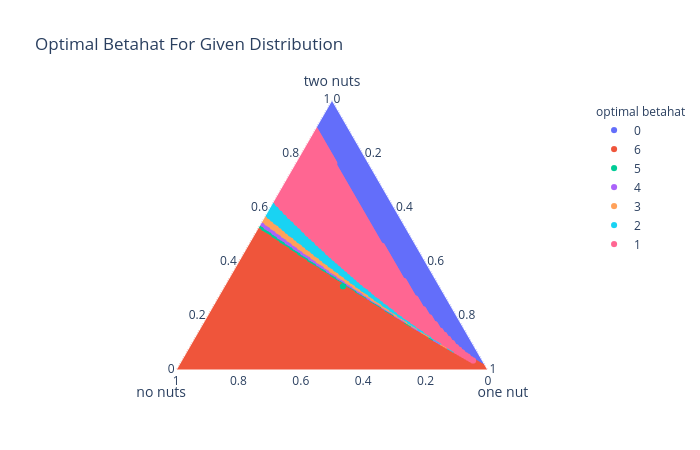
\includegraphics[scale = 0.8]{optimal_betahat_Aug17} \\
\end{figure}
\begin{figure}[H]
    \centering
    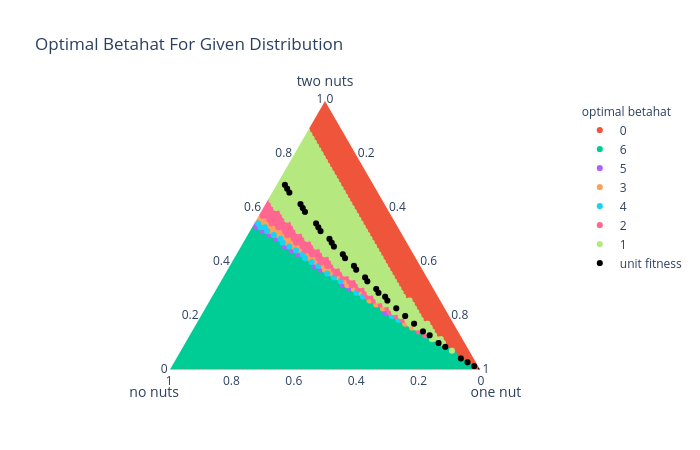
\includegraphics[scale = 0.8]{overlaid_unit_fitness} \\
\end{figure}
\begin{figure}[H]
    \centering
    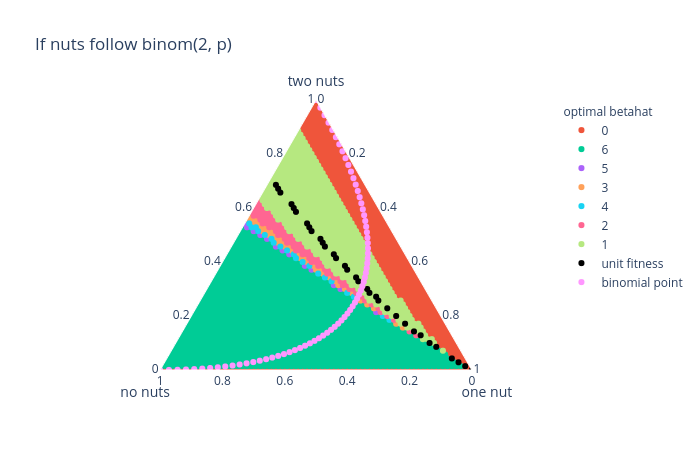
\includegraphics[scale = 0.8]{overlaid_binom} \\
\end{figure}
\begin{figure}[H]
    \centering
    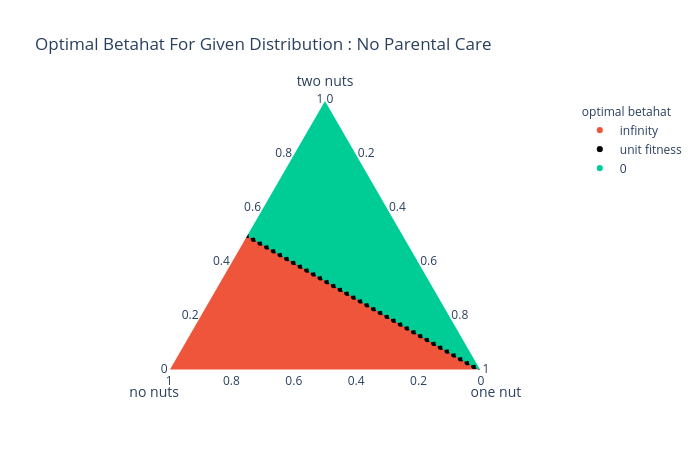
\includegraphics[scale = 0.8]{unit_fitness_no_pc} \\
\end{figure}


Courtesy of Jaye's suggestion, I'll start using the terminology Parental Care for what has until now been called ``pregnancy.'' 
The idea right now is to get some intuition for why squirrels make the decisions they do. Of course, we have computed the different
fitnesses and thus the optimal $\hat \beta$ is indisputable, but the indifference arcs (for example, between $\hat \beta = 0, 1$) seem
to be drawn arbitrarily. Why are those arcs where they are? And can we get some intuition for why exactly we need ever increasing
values of $\hat \beta$ to fill the entire half of the simplex with $p_2 > p_0$?  \\ \\
Fitness can be thought of as defined by
$$ r = 1 + b - d $$
where $b,d$ are respectively the birth and death rates of the population. Take as given a demographic matrix $L$, its leading eigenvalue
$r$, and its corresponding eigenvector $\left( n_0, n_1, \ldots, n_{\hat \beta}, n_{PC} \right)$ normalized
such that $\sum n_k = 1$. In a given time step, we can expect that anybody surviving the period of parental care gives birth; at the same time,
any squirrel with zero nuts banked and who finds zero nuts will die. This gives
\begin{itemize}
    \item $b = n_{PC}$ or $b = (1 - p_0)n_{PC}$ if $\hat \beta = 0$,
    \item $d = n_0p_0$.
\end{itemize}
In sum,

$$ r_{\hat \beta} =
\begin{cases}
    1 + n_{PC}^{\hat \beta}\left( 1 - p_0 \right) - n_0^{\hat \beta}p_0 & \text{ if  } \hat \beta = 0 \\
    1 + n_{PC}^{\hat \beta} - n_0^{\hat \beta}p_0 & \text{ if  } \hat \beta \ge  1
\end{cases}
$$

%Notice $n_{PC} = p_2 n_{\hat \beta}$, so
%$$ r_{\hat \beta} =
%\begin{cases}
%    1 + p_2n_{\hat \beta}^{\hat \beta}\left( 1 - p_0 \right) - n_0^{\hat \beta}p_0 & \text{ if  } \hat \beta = 0 \\
%    1 + p_2n_{\hat \beta}^{\hat \beta} - n_0^{\hat \beta}p_0 & \text{ if  } \hat \beta \ge  1
%\end{cases}
%$$
Intuitively, increasing $\hat \beta$ decreases the value of each $n_k$. The intuition is that increasing the number
of bins decreases how much we can put in each bin. 
%For each increase in $\hat \beta$, we (experimentally) find
%that $n_{PC}$ decreases by about half as much as $n_0$. 
To gain an intuitive appreciation for the positioning of the indifference
arcs, consider the following. Assume $\hat \beta \ge 1$ (so we don't have to deal with the $\hat \beta = 0$ case from above). Then:

\begin{align*}
    r^{\hat \beta} \le r^{\hat \beta + 1} &\iff  n_{PC} - p_0n_0 \le n_{PC}' - p_0n_0' \\
    &\iff n_{PC} - n_{PC}' \le p_0\left( n_0 - n_0' \right) \\
    &\iff \frac{n_{PC} - n_{PC}'}{n_0 - n_0'} \le p_0
\end{align*}

The above is a bit notationally dense. We use primes to denote the leading eigenvector of $L_{\hat \beta + 1}$; that is,
$n$ is such that $L_{\hat \beta} n = r^{\hat \beta}n$ and $n'$ is such that $L_{\hat \beta + 1}n' = r^{\hat \beta + 1}n'$. 
We therefore have a condition for choosing to save to $\hat \beta + 1$, given our position in the simplex: compute 
$$ f\left( p_0, p_1, \hat \beta \right) := \frac{ \Delta n_{PC}}{\Delta n_{0}} $$
and compare with the constant $p_0$.  \\ \\

Another tangent. It is clear upon reflection that $n_{PC} = \frac{p_2 n_{\hat \beta}}{r_{\hat \beta}}$. Then 
\begin{align*}
    r &= 1 + n_{PC} - p_0n_0 \\
    r &= 1 + \frac{p_2 n_{\hat \beta}}{r} - p_0 n_0 \\
    r^2 &= (1 - p_0n_0)r + p_2n_{\hat \beta} \\
    0 &= r^2 + \left( p_0n_0 -1 \right)r - p_2n_{\hat \beta},
\end{align*}
to which we can apply the quadratic formula to obtain
$$ r = \frac{ 1 - p_0n_0 \pm \sqrt{\left( 1 - p_0n_0 \right)^2 + 4p_2n_{\hat \beta}}}{2}. $$
Since $n_k\to0$ for each $k$ as $\hat \beta\to \infty$, we can conclude that 
$r\to0, 1$ as $\hat \beta\to \infty$. This, after some thought, is intuitive; if an infinitely large population of squirrels
somehow managed to get to stable savings distribution, then almost nobody dies and almost nobody reproduces, so that the population remains
stable irrespective of the distibution of nuts.  \\\\

We can leverage the quadratic formula expression above to get a nice result. We have $r_{\hat \beta} > 1$ iff
\begin{align*}
    \frac{ 1 - p_0n_0 + \sqrt{(1 - p_0n_0)^2 + 4p_2n_{\hat \beta}}}{2} &\ge 1 \\
    \sqrt{(1 - p_0n_0)^2 + 4p_2n_{\hat \beta}} &\ge 1 + p_0n_0 \\
    (1 - p_0n_0)^2 + 4p_2n_{\hat \beta}  &\ge \left( 1 + p_0n_0 \right)^2 \\
    4p_2n_{\hat\beta} &\ge 4p_0n_0 \\
    p_2n_{\hat\beta} &\ge p_0n_0
\end{align*}

The above expression agrees with my historic intuition. I \textit{wanted} to say that $n_{PC} = p_2n_{\hat \beta}$, but that,
it turns out, is false. But we get the exact same condition for $r_{\hat \beta} > 1$ as if it did hold. Cool!


\section{Measure Theoretic Approach}

Assume a discrete time setup $t\in\N$.
Suppose at time $t = 0$ we have a population consisitng of $i\in\left\{ 1, 2, \ldots, I \right\}$ individuals,
each of age $a_i\in\N$. Suppose offspring production is a random process,
iid between individuals, determined by age $a$; that is, $X(a)$ is the random variable specifying the number of offspring produced, or $-1$ if 
the individual dies. Then the population the following time step is 
$$ \text{pop}(1) = I + \sum\limits_{i = 1}^I X_i(a_i).$$
More poignantly, the \textit{relative} population size is:
$$\frac{1}{I}\text{pop}(1) = 1 + \frac{1}{I}\sum\limits_{i = 1}^I X_i(a_i)$$
Perhaps even \textit{MORE} poignantly, the relative population size in expectation is:
\begin{align*}
    E\left[\frac{1}{I}\text{pop}(1)\right] &= 1 + \frac{1}{I}\sum\limits_{i = 1}^I g(a_i) \\
    &= 1 + \int_0^\infty g(a) d\mu(a)
\end{align*}
where $g$ is the offspring minus death mass function and $\mu$ is the distribution on
$\N$ specifying the proportion of the population in each age class $a\in\N$. We generalize immediately,
and claim that in discrete time, fitness is defined by:
$$ r = 1 + \sum\limits_0^\infty g(a) \mu(a) = 1 + \int_0^\infty g(a) d\mu(a), $$
where once more $g$ is the birth density function minus the death density function, and $\mu$ is a probability
measure on $\R_{> 0}$ specifying the distribution of the population. Generalizing even further, the population growth rate
is just
$$ \int_0^\infty g(a) d\mu(a) $$
which applies equally to continuous and discrete time models. So are we done? Of course not! Look at how much is left to be read on
the next page! Continue with discrete time as our motivating set up; everything will (hopefully) translate well enough to continuous
time. We began with a distribution $\mu$ providing the fraction of the population in each age category; call it $\mu_0 = \mu$. After
everybody gives birth and gets older, we have a new age distribution, $\mu_1$. Concretely,
$$ \mu_1(a) = 
\begin{cases}
    \sum\limits_0^\infty g(a) \mu_0(a) & \text{ if  } a = 0 \\
    (1 - \delta(a-1))\mu_0(a-1) & \text{ else.}
\end{cases}
$$
In the above, $\delta(\cdot)$ is the function specifyiing the probability of dying at age $a$, so that $1-\delta$ is survival probability.
To make $\mu_1$ a probability measure, we need to rescale so that $\mu_1(\R) = 1$; set $\mu_1 = \frac{1}{r_1}\mu_1$. We can similarly define
$\mu_t$ recursively for each $t\in\N$. A natural question is: does our age distribution stabalize down to something nice? That is, does
$\mu_t(a)\to \nu(a)$ for each $a\in\N$? 

\subsection{For concreteness, Leslie matrices as an example}
Everything above was highly abstract; how am I so convinced that what I've written is correct? Fortunately, the Leslie model 
encorporates all of the elements above, and so allows us to check: does this all okay? Suppose we have three age classes,
$a\in\left\{ 0, 1, 2 \right\}$, survival probabilities $s_0, s_1, s_2 = 0$, and birth rates $b_0, b_1, b_2$. This setup produces the
standard Leslie matrix:
$$ L = 
\begin{pmatrix}
    b_0 & b_1 & b_2 \\
    s_0 & 0 & 0 \\
    0 & s_1 & 0 \\
\end{pmatrix}
$$
Translating to the setup above, we have $g(a) = b_a - s_a$. As per standard Leslie model stuff, we have a stable age distribution:
call it $(n_0, n_1, n_2)$. By setting $\mu(a) = n_a$, we can experimentally check: does
$$ \sum g(a)\mu(a) = r$$
where $r$ is the leading eigenvalue of $L$? I checked and it worked once, so I figure yes, it must hold in general. 

\subsection{Back to abstract measure theory stuff}
What we are looking at very closely resembles a Markov chain. I'm hopeful that we can co-opt the tools from Markov Chain Theory to
prove that under analogous conditions to aperiodicity, there exists a unique stationary measure $\mu$ for our population growth
process to which the $\mu_t$ converge (what exactly is meant by convergence is to be determined).  
\subsection{Corrections}

Last week, I told some lies, which I will now try to rectify. On the one hand, if $\beta, \delta$ are instantaneous birth and
death rates as a function of age (assuming we have reached a given age), then we do indeed have:
$$ r = \int_0^\infty (\beta(a) - \delta(a))d\mu(a) = \int_0^\infty(\beta(a) - \delta(a))n(a) da. $$
We can get away from using a measure $\mu$ to multiplying by the stable age distribution due to Radon-Nikodym. The picture I tried
to use to motivate all of this work is slightly different. The graph showing the ``typical life history'' of a squirrel actually corresponds
to the function $\beta(a)\cdot s(a)$, where $\beta$ is as above and $s$ is the probability of surviving to age $a$. Then the question is:
for what measure $\Delta$ does 
$$ \int_0^\infty \beta(a) s(a) d \Delta(a)?$$
We use $\Delta$ for discounting, since $\delta$ is already used for the instantaneous death rate. By a simple re-arrangement, we can write
\begin{align*}
    r &= \int (\beta(a) - \delta(a))n(a) da \\
    &= \int \beta(a) s(a) \frac{\beta(a) - \delta(a)}{\beta(a) s(a)} n(a) d a.
\end{align*}
So interestingly, we can take
$$ \Delta(a) = \frac{\beta(a) - \delta(a)}{\beta(a) s(a)} n(a).  $$
``Why is this interesting?'' you might ask. Well, for one thing $\Delta(a) < 0$ whenever $\beta < \delta$. Further, $\Delta$ need not be
decreasing. Nevertheless, this is something to work with.



\subsection{Examples of life history displays}
For the sake of concreteness, as well as tying squirrel banking together with this abstract nonsense, we can compute
the expected life history of a squirrel saving to different $\hat \beta$. In particular, for $(p_0, p_1, p_2) \approx
(0.1089, 0.4725, 0.4186)$, we have the following life histories:

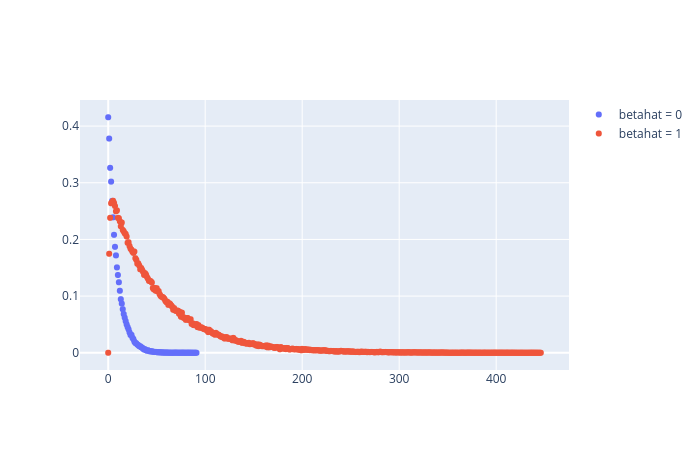
\includegraphics[scale = 0.8]{life_histories} \\

We chose these values for $p_0,p_1, p_2$ because at this distribution of nuts, the fitness for $\hat \beta = 0$ is about the same
as that of $\hat \beta = 1$. 
Each point represents the expected number of offspring a squirrel produces on a given day in its life, with the horizontal axis being
time. Below, it is more zoomed in.

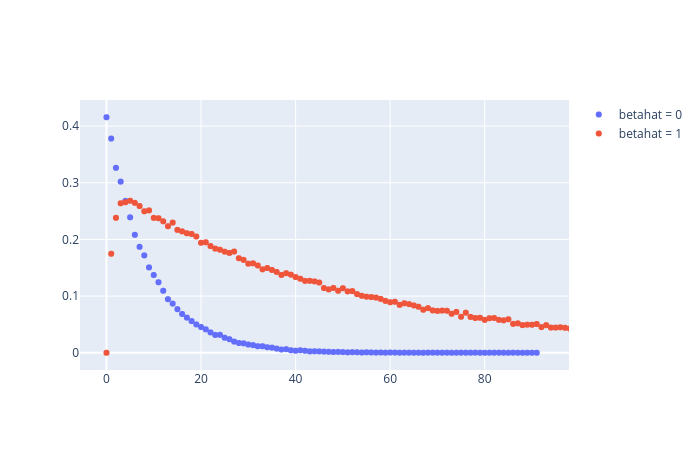
\includegraphics[scale = 0.8]{zoomed_life_histories} \\

\subsection{Summing up all contributions}
I am still pathologically trying to get life history to tell a discounting story. In particular, I want to find a 
discounting function $\Delta(a,q)$ satisfying
$$ \int_0^\infty \beta(a) s(a) \Delta(a, \beta(a) s(a)) d a = \text{ fitness.} $$
In what follows, $q$ can be thought of as ``quantity of offspring produced.'' For any measure of fitness, we have
$$ \text{fitness } = \text{ fitness}(q_{1}, q_{2}, \ldots ),$$
with $q_a$ the quantity of offspring at age $a$. Let's assume (and this is a significant assumption) that we can decompose the different
contributions to fitness as 
$$ \text{fitness } = \sum\limits_{a = 1}^\infty C(a, q_a),$$
with $C(a, q_a)$ representing the total contribution to fitness of quantity $q_a$ at age $a$. This is a significant assumption since it
implies that
$$ \frac{\partial}{\partial q_{a}} \text{fitness } = \frac{\partial}{\partial q_{a}} C(a, q_a). $$
In particular, varying the quantity you produce on a given day does not impact the contribution to fitness on other days. This seems sort of
unreasonable, but we proceed nevertheless. By the fundamental theorem of calculus, we know that
$$ C(a, q_a) = \int_0^{q_a} \frac{\partial}{\partial q} C(a, q) d q = q_a \mathbb{E}_0^{q_a}\left[ \text{MCF}_a \right]. $$
In the above, $\text{MCF}_a$ is the marginal contribution to fitness. Plugging this into our expression for fitness, we have
$$ \text{fitness } = \sum\limits_{a = 1}^\infty q_a \mathbb{E}_0^{q_a}\left[ \text{MCF}_a \right].$$ 
Thus taking $\Delta(a, q_a) = \mathbb{E}_0^{q_a}\left[ \text{MCF}_a \right]$ produces a discounting function which gives back
fitness. \\\\

\textbf{Pure Leslie Matrix analysis} \\\\

Assume a Leslie model setup: we have a maximal age of $A \le \infty$, day to day survival probability is $s_1, s_2, \ldots, s_{A-1}$,
and fecundity is $b_1, b_2, \ldots, b_A$. The Euler-Lotka equation is:

$$ \lambda^A = \sum\limits_{a = 1}^A \lambda^{A-a}s_1 s_2 \cdots s_{a-1} b_a.$$

We can use implicit differentiation (or the semi-valid $\frac{\d \lambda}{ \d b_\alpha} = \frac{\d EL}{\d b_\alpha}/
\frac{\d EL}{\d \lambda}$) to obtain:

\begin{align*}
    \frac{\d \lambda}{\d b_{\alpha}} &= \frac{\lambda^{A-\alpha}s_1s_2\cdots s_{\alpha-1}}{A\lambda^{A-1} -
    \sum\limits_{a = 1}^{A-1}s_1s_2\cdots s_{a-1}b_a\lambda^{A-a-1}} \\\\
    &= \frac{\lambda^{A-\alpha}}{\lambda^{A-1}} \cdot \frac{s_1s_2\cdots s_{\alpha-1}}{A - \sum\limits_{a = 1}^{A-1}s_1s_2\cdots s_{a-1}b_a\lambda^{-a}}\\\\
    &= \lambda^{1-\alpha} \cdot \frac{s_1s_2\cdots s_{\alpha-1}}{A - \sum\limits_{a = 1}^{A-1}s_1s_2\cdots s_{a-1}b_a\lambda^{-a}},
\end{align*}
where $\alpha\in\left\{ 1, 2, \ldots, A \right\}$ is arbitrary. This seems to be getting us nowhere! Nevertheless, we continue by
noting that $\frac{\d \lambda}{\d b_\alpha} = \text{MCF}_\alpha$, so that our proposed discounting function above turns out to be:

\begin{align*}
    \Delta(\alpha, q(b_\alpha)) &=\frac{1}{q(b_{\alpha})} \mathbb{E}_0^{q(b_\alpha)}\left[ \text{MCF}_\alpha\right] \\
    &= \frac{1}{q(b_{\alpha})} \int_0^{q(b_\alpha)} \lambda^{1-\alpha} \cdot \frac{s_1s_2\cdots s_{\alpha-1}}{A - \sum\limits_{a = 1}^{A-1}s_1s_2\cdots s_{a-1}b_a\lambda^{-a}} \d b_\alpha \\
    &= \frac{\lambda^{1-\alpha}}{s_1s_2\cdots s_{\alpha-1}b_{\alpha}}\cdot\int_0^{q(b_\alpha)} \frac{s_1s_2\cdots s_{\alpha-1}}{A - \sum\limits_{a = 1}^{A-1}s_1s_2\cdots s_{a-1}b_a\lambda^{-a}} \d b_\alpha \\
    &= \frac{\lambda^{1-\alpha}}{b_{\alpha}}\cdot\int_0^{q(b_\alpha)} \frac{1}{A - \sum\limits_{a = 1}^{A-1}s_1s_2\cdots s_{a-1}b_a\lambda^{-a}} \d b_\alpha \\
\end{align*}

This is starting to look like something more interesting - of particular note is the fact that we have an exponential discounting term $\lambda^{1-\alpha}$
floating around in there. For sufficiently large $b_{\alpha}$, notice that $\lambda\to\infty$ so that $\lambda^{-a}\to 0$ for each 
$a\in\left\{ 1, 2, \ldots, A-1 \right\}$. Thus, for $b_\alpha$ sufficiently large, the integrand begins to look like

\begin{align*}
    \int_0^{q(b_\alpha)} \frac{1}{A - \sum\limits_{a = 1}^{A-1}s_1s_2\cdots s_{a-1}b_a\lambda^{-a}} \d b_\alpha &\to  \int_0^{q(b_\alpha)} \frac{1}{A} \\
    &= q(b_\alpha)\frac{1}{A} \\
    &=  \frac{s_1 s_2 \cdots s_{\alpha-1} b_\alpha}{A}.
\end{align*}
Substituting back into the original expression for the discounting function $\Delta(\alpha, q)$, we get

\begin{align*}
    \Delta(\alpha, q(b_\alpha)) \to \frac{\lambda^{1-\alpha}s_1 \cdots s_{\alpha-1}}{A}.
\end{align*}
If we further assume that survival probability is constant (say $s_a = s$ for all $a$), we obtain

$$ \Delta(\alpha, q(b_\alpha)) \to \frac{1}{A}\left( \frac{s}{\lambda} \right)^{1-\alpha}\sim \left( \frac{s}{\lambda} \right)^{-\alpha} $$








\section{Playing with survival rates}
Exponential discounting comes from perhaps the simplest model imaginable. A squirel should be indifferent
between two findings whenever they are equal in expected value. If a squirrel has geometric survival (with parameter
$s$), then a future payment $F_t$ (at time $t$) is, in expectation, $s^t F_t$. I now ask: what survival rates give
hyperbolic discounting? 
\begin{itemize}
    \item At $t = 1$, we require $\frac{1}{1 + h} = s_0$. Rearranging gives $h = \frac{1 - s_0}{s_0}$. 
    \item By induction we can show that $s_0\cdot s_1 \cdot \ldots \cdot s_t = \frac{1}{1 + ht}$ whenever
        $s_a = \frac{ (a - 1) - (a - 2)s_0}{a - (a - 1)s_0}$. 
\end{itemize}
For instance, if initial survival is $s_0 = 1/2$, then survival must grow according to $s_a = \frac{a+1}{a+2} = \frac{2}{3}, \frac{3}{4}, 
\frac{4}{5},\ldots$ in order for a squirrel to discount hyperbolically in the simplistic model wherein a future payment is equal to
its expected value.

\subsection{Age structured model}
Fix squirrels with  birth and survival distributions $b_0, \ldots, b_A$ and $s_0, \ldots, s_{A-1}$, leading to a Lyapunov exponent
of $\lambda_0 = \lambda(b, s)$. The experimental approach of offering a payment of $P$ immediately and increasing/decreasing future payments $F_t$ until
indifference can be closely approximated.
\begin{enumerate}
    \item Increase initial fecundity $b_0$ to $b_0 + P$. 
    \item Compute $\lambda' = \lambda(b_0 + P, \text{ all else same }) $. 
    \item Determine $F_1$ such that $\lambda(b_0, b_1 + F_a, b_2, \ldots) = \lambda'$. Interpretation: a squirrel is fitness
        indifferent between a payment of $P$ at age $0$ and $F_1$ at age $1$.
    \item Repeat for $a = 2, \ldots, A$. 
    \item The resulting list $\left[ P, F_1, F_2, \ldots, F_A \right]$ tracks the required appreciation of $P$ for indifference.
\end{enumerate}
The expected payout model predicts that appropriately increasing survival should lead to hyperbolic discounting \textit{
independent of fecundity}. How does this hold up in practice?
Take $A = 10$, and $s = [1/2, 2/3, 3/4, 4/5, 5/6, 6/7, 7/8, 8/9, 9/10, 10/11]$. For simplicity, the birth vector
will be $\left[ b, b, b, \ldots, b \right]$. The population has age independent fecundity. We vary $b$ in order to understand
the appreciation trend of an initial payment of $0.01$. We find that the most important difference is whether $\lambda_0 \lessgtr  1$. 
\begin{figure}[H]
    \centering
    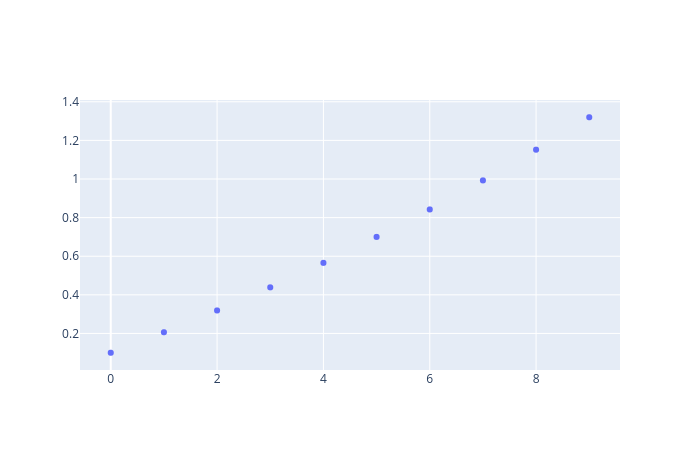
\includegraphics[scale = 0.7]{reqd_fec_increase_unit_fitness.png}
    \caption{Appreciation of 0.1 for a life history with $\lambda_0 = 1$.}
\end{figure}
\begin{figure}[H]
    \centering
    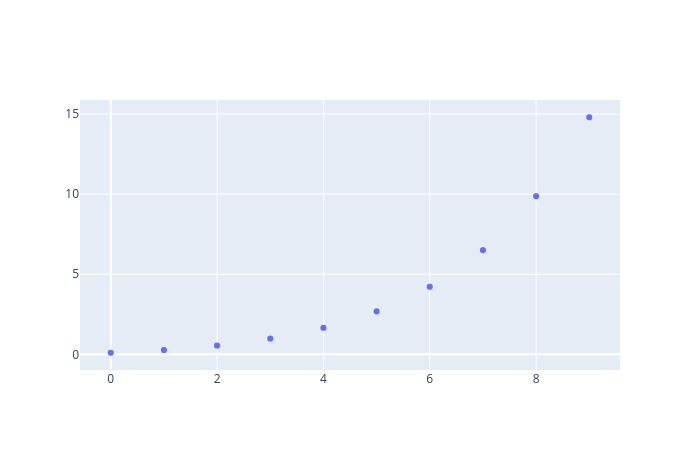
\includegraphics[scale = 0.7]{reqd_fec_increase_fitness_ge1.png}
    \caption{Appreciation of 0.1 for a life history with $\lambda_0 = 1.3 > 1$.}
\end{figure}
\begin{figure}[H]
    \centering
    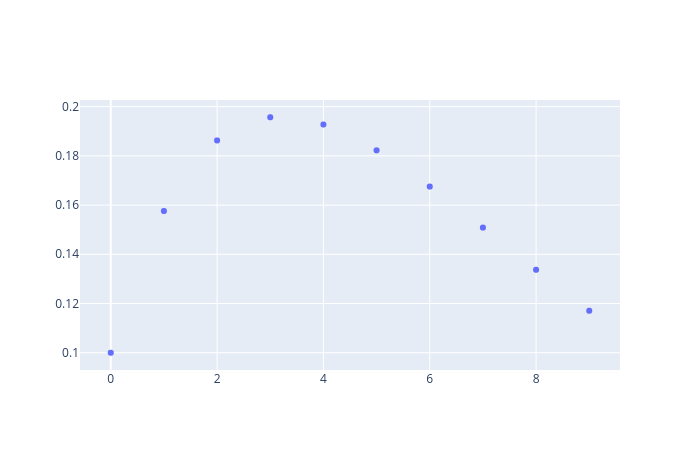
\includegraphics[scale = 0.7]{reqd_fec_increase_fitness_le1.png}
    \caption{Appreciation of 0.1 for a life history with $\lambda_0 = 0.75 < 1$.}
\end{figure}
This seems fantastic. Can I give some kind of analytic rationale for why such richness in discounting schemes? It runs out we have
done enough work already to understand. Remember that 
$$ \frac{\d \lambda}{\d b_{\alpha}} \approx \lambda^{-\alpha}\cdot \left( s_0\cdot\ldots\cdot s_{\alpha - 1} \right)$$
where $\approx$ is taken to mean both approximately equal and proportional to (proportionality doesn't matter - we can scale a discounting
function by any constant, since only relative size matters). If $\lambda = 1$, we get exactly the simplistic expected payment model.
If $\lambda > 1$, we have a product of exponential and hyperbolic discounting, and the exponential term will tend to dominate. Finally,
if $\lambda < 1$, we have negative exponential discounting at the same time as hyperbolic discounting. The exponential term will tend to
value \textit{future payments more heavily than present value}, explaining the $\cap$ shape we see in the third figure. 
Our analysis is really only valid for marginal increases in $b_0$. Too large an increase will push $\lambda \gg 1$, and the exponential
term will again dominate.
\begin{figure}[H]
    \centering
    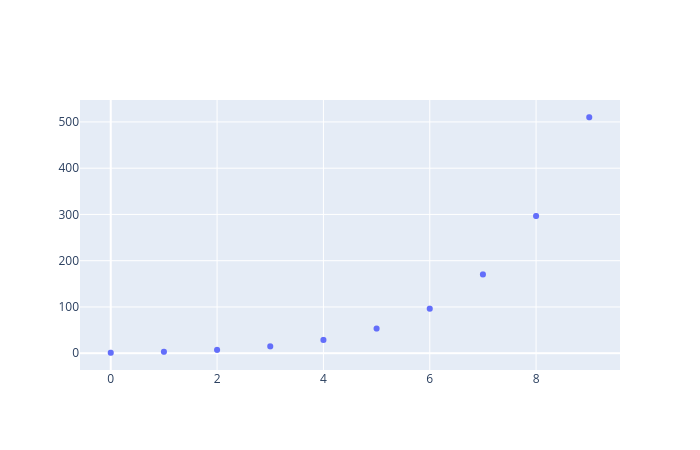
\includegraphics[scale = 0.7]{reqd_fec_increase_bigP.png}
    \caption{Appreciation of 1 for a life history with $\lambda_0 = 1$.}
\end{figure}
We can get creative, however, and vary $\lambda$ to compensate for a big $P$ so as to still come away with hyperbolic discounting. 
 \begin{figure}[H]
    \centering
    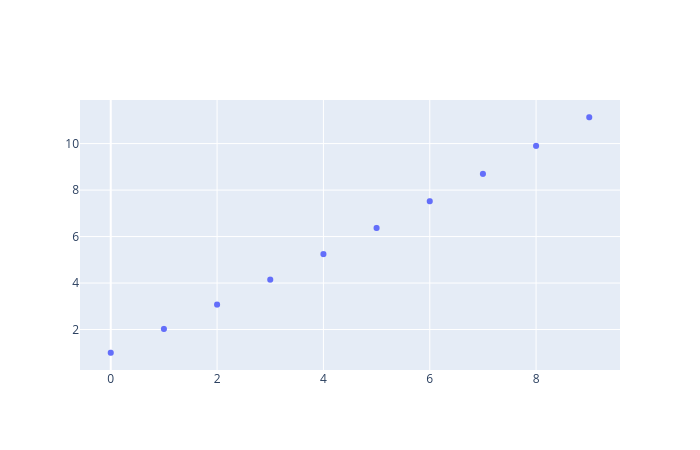
\includegraphics[scale = 0.7]{reqd_fec_increase_bigP_low_fitness.png}
    \caption{Appreciation of 1 for a life history with $\lambda_0 = 0.5$.}
\end{figure}  
\subsection{A conspiracy theory}
It took me a while to remember from where I recognized the sequence $\frac{1}{2}, \frac{2}{3}, \frac{3}{4}, \ldots$. Do you remember?
It actually came about earlier in this document, when discussing increasing survival as a squirrel's cache of nuts increases. 
Briefly, two nuts were found daily, and a squirrel has survival $s_{\beta}$ when it has $\beta$ nuts saved. A question I asked at 
the time was: For what values of $s_0, s_1, \ldots, s_{\hat \beta}$ does a squirrel have unit fitness? It turns out that
the same pattern as leads to hyperbolic discounting leads to unit survival in the increasing survival with banked nuts model. 
At a high level:
\begin{enumerate}
    \item Looking for unit fitness $\Rightarrow$ $s = \frac{1}{2}, \frac{2}{3}, \frac{3}{4}, \ldots$
    \item Looking for hyperbolic discount $\Rightarrow$ $s = \frac{1}{2}, \frac{2}{3}, \frac{3}{4}, \ldots$
\end{enumerate}
We have what seems to be an awfully big coincidence here. To quote Jaye, who was quoting someone else, ``correlation does not
imply causation, but it does imply unresolved causal structure.'' I want to find that structure! Is it possible that unit
fitness and hyperbolic discounting go hand in hand? I can rule that out: if $s_a$ is constant and $b$ is such that $\lambda = 1$,
then we will still have exponential discounting. I'm rambling, but this is interesting to think about.





\section{Total Reproductive Output}
Christoph sends the following in an email: \\ \\

``\ldots wondering whether it is even necessary to try to tie everything back to Lyapunov exponents in Leslie matrices. 
Instead, I think all that is needed is to calculate the lifetime reproductive output of an individual (which follows from 
your graphs). This is an excellent measure of fitness. The only challenge is the comparison between individuals with different life histories and, 
in particular, different life expectancies. A reasonable approximation would be to raise the fitness of the shorter lived 
type to some power that depends on the ratio of the two life expectancies.'' \\ \\

Here is a first attempt: denote by $\int \text{LH}(a) \d a$ = RR the total expected number of offspring for an individual with life history
LH, and as a (terrible) shorthand, denote $\mathbb{E}$ its life expectency. Propose the following measure of fitness:

$$ f := \left( \int \text{ LH} (a) \d a \right)^{\frac{1}{\mathbb{E}}}.$$

This looks to be somewhat arbitrary, but it actually has some nice properties.

\begin{itemize}
    \item Not replacing oneself leads to fitness $< 1$ irrespective of the life expectancy, since $r^x < 1$ for all $r\in(0,1)$ and
        $x > 0$. 
    \item Low life expectancies with replacement rate $> 1$ are rewarded; if $r > 1$ and $\mathbb{E}$ is large, then we have something
        of the form $r^x$ where $x$ is large, which blows up pretty quickly. 
    \item Comparing a smaller/sooner with a larger/later life history yields exactly the ratio of life expectancies referenced in 
        Christoph's email:
        \begin{align*}
            f_{\text{SS}} = f_{\text{LL}} &\iff \left( \text{RR}_{\text{SS}} \right)^{\frac{1}{\mathbb{E}_{\text{SS}}}} =
                \left( \text{RR}_{\text{LL}} \right)^{\frac{1}{\mathbb{E}_{\text{LL}}}} \\
                &\iff \left( \text{RR}_{\text{SS}} \right)^{\frac{\mathbb{E}_{\text{LL}}}{\mathbb{E}_{\text{SS}}}} = \text{RR}_{\text{LL}}
        \end{align*}
\end{itemize}


\section{Moran Squirrels}
Consider a Moran birth-death process with two types $A$ and $B_T$. Type $A$ has constant fitness $1$, whereas type $B_T$ has
fitness determined by its age.
$$ \text{Fitness of individual of type }B_T =
\begin{cases}
    0 & \text{if age }<T \\
    \beta & \text{if age }\ge T
\end{cases}
$$
A population consisting of exclusively $A$ types is boring. A popultion consisting of exclusively $B_T$ types is marginally more interesting,
in that we can ask: does it reach a stable age distribution? By induction (or something, I've yet to sort out all of the details, but
it definitely works), a population of size $N$ has stable age distribution:
$$\left( n_0, n_1, \ldots, n_{T-1}, n_{\ge T} \right) = \left( 1, s, s^2, \ldots, s^{T-1}, \sum\limits_{t = T}^\infty s^t \right)$$
where $s = 1 - \frac{1}{N}$ is survival probability. For $N < \infty,$ this is just an approximation, since there will necessarily be some
stochastic fluctuations. With this stable age distribution, we can determine that
\begin{align*}
    \text{Average fitness of }B_T\text{ types } &= \frac{0\cdot n_{<T} + \beta\cdot n_{\ge T}}{n_B} \\
    &= \frac{\beta \cdot \frac{s^T}{1-s}}{\frac{1}{1-s}} \\
    &= \beta s^T
\end{align*}
Recall: this was all just for the case of a population consisting exclusively of $B_T$ types. If we throw in a mixture of $A$ types
and $B_T$ types, it is not obvious how this will impact the stable age distribution of $B_T$ types. Nevertheless, if we assume that
they hover around
$$\left( n_0, n_1, \ldots, n_{T-1}, n_{\ge T} \right) = \left( y, ys, ys^2, \ldots, ys^{T-1}, \sum\limits_{t = T}^\infty ys^t \right)$$
where $y$ is some constant, we find the exact same result:
$$\text{Average fitness of }B_T\text{ types } = \beta s^{T}.$$
We perform a system size expansion. With notation as in Evoludo.pdf, 
\begin{itemize}
    \item $T^+(x) = P\left( A \text{ type dies} \right)\cdot P( B \text{ type rep.}) = (1-x)\cdot \frac{\beta s^T x}{(1-x) + \beta s^T x}$
    \item $T^-(x) = P\left( B \text{ type dies} \right)\cdot P( A \text{ type rep.}) = 
        x\cdot \frac{1 - x}{(1 - x) + \beta s^T x}$,
\end{itemize}
so that the general tendency of the system is neutral (resp. in favour of $A$, $B_T$ types) whenever $T^+ - T^- = 0$, that is, whenever
$1 - s^{T} = 0$ (resp $>0, <0$). 
By system size expansion, large $N$, etc. etc., so on and so forth, $A$ types and $B_T$ types can coexist in infinite populations whenever
\begin{align*}
    1 = \beta s^{T} &\iff \beta = s^{-T}
\end{align*}
Thus in some sense, Moran squirrels discount exponentitally with discounting parameter $s$. It is reasonable to wonder: if $A$ and $B$ types
survive with different probabilities, then how does this impact discounting behaviour? Answer: the daily double. We need to be careful how we set
up the system. To encode that $B_T$ types are less (resp. more) susceptible to death than $A$ types, we introduce susceptibility parameter $u < 1$
(resp. $> 1$). The individual to die is selected with probability proportional to its susceptibility, so that we have
\begin{itemize}
    \item $T^+(x) = P\left( A \text{ type dies} \right)\cdot P( B \text{ type rep.}) = \frac{1-x}{(1-x) + ux}\cdot \frac{\beta s^T x}{(1-x) + \beta s^T x}$
    \item $T^-(x) = P\left( B \text{ type dies} \right)\cdot P( A \text{ type rep.}) = 
        \frac{ux}{(1-x) + ux}\cdot \frac{1 - x}{(1 - x) + \beta s^T x}$.
\end{itemize}
Just as above, the general tendency of the system is neutral whenever $T^+ - T^- = 0$, which occurs precisely when 
$$ \beta s^T = u \iff \beta = u\cdot s^{-T}.$$

\section{Squirrelly Bandits}
For Christoph's Math564, I did a project called Squirrelly Bandits. I did a writeup, so see there for the details. Broadly,
I was surprised to find that the evolutionary objective of optimizing fitness is equivalent to a reinforcement learning
objective via appropriate choice of discounting parameter. Specifically, I find \textit{numerical} evidence that
$$ arg\max_{\varepsilon} \text{ Leading E-val of }B_{\varepsilon} = 
arg\max_{\varepsilon} \sum\limits_{t = 0}^\infty \gamma^t \mathbb{E}_{\varepsilon}\left[ r_t \right].$$
In words: the evolutionary objective of fitness maximization can be made equivalent to an RL objective by appropriate choice of 
opportunity cost parameter. I have figured out why this is the case, and what the ``appropriate'' $\gamma$ is. \\ \\

Notice that the stable age distribution of a population with inifinitely many age classes (also holds for finitely many, but
it's a little bit more work notationally):
$$ (n_0, n_1, n_2, n_3, \ldots) = (\Sigma, s_0 n_0, s_1 n_1, s_2 n_2, \ldots)\frac{1}{R} $$
where $R$ is the per time step growth rate. Then $n_1 = R^{-1} s_0 n_0$, $n_2 = R^{-1} s_1n_1 = R^{-2} s_0s_1 n_0 $, and so forth. 
Recall that fitness $\lambda$ satisfies
$$ \lambda = \sum\limits_{a = 0}^\infty n_a \cdot b_a $$
where $b_a$ is fecundity at age $a$. In this case, then, we have
$$ \lambda = n_0\sum\limits_{a = 0}^\infty s_0 \cdots s_{a-1} R^{-a} \mathbb{E}\left[ r_t \right].$$
So if survival probability is constant, as it is in squirrel banking, then by taking $\gamma = s/R$, we have that the objective of
maximizing $\sum \gamma^t \mathbb{E}\left[ \hat r_t \right]$ maximizes fitness, where $\hat r_t$ is the reward at time $t$ conditional
on still being alive. As an extension, even if survival probability were not constant,
it wouldn't matter. Just bake survival into the expectation, rather than making it conditional on still being alive, and you have an opportunity
cost parameter $\gamma = 1/R$. 


\newpage
\bibliographystyle{alpha}
\bibliography{research}{}






\end{document}



